\documentclass[a4paper]{article}
\usepackage[utf8]{inputenc}
\usepackage{graphicx}

\begin{document}

\section{Vererbung}

Gregor Mendel (1822 - 1884) war zuständig für den Klostergarten (Mönch). Er hat zufällig Erbsen in verschiedenen Farben gepflanzt. Er hat nun verschiedene Farben miteinander gekreuzt, um zu sehen was passiert.
\newline
\newline
Unformitätsregel:
\newline
\newline
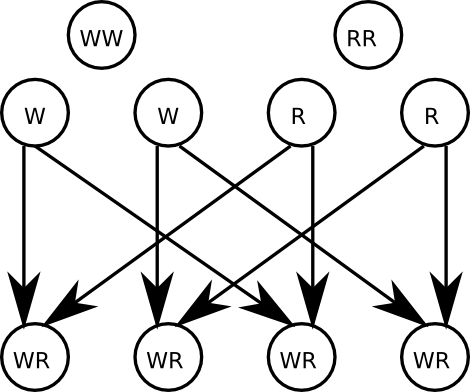
\includegraphics[scale=0.25]{image/1.png}
\newline
\newline
Spaltungsregel:
\newline
\newline
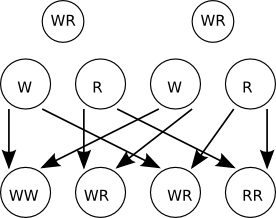
\includegraphics[scale=0.75]{image/2.png}
\newline
\newline
Die Kinder von reinrassingen Eltern sind Mischlinge. Genotypus sind alle gespeicherten Merkmalen in der Zelle. Phenotypus sind alle ausgebildeten Merkmale. Merkmale können rezessiv oder dominat sein. Dominante Merkmale setzten sich bei Kreuzungen mit rezessiven Merkmale durch und werden ausgebildet. Die Körperzelle hat alle Merkmale doppelt gespeichert (nennt man Diploid). Die Geschlechtszellen haben die Merkmale nur einmal gespeichert (nennt man Happloid).
\newline
\newline
Die Bluterdkrankheit kann sich bei Inzucht besonders gut weiterbilden. Der Mann erkrankt jedoch leichter als die Frau, da Männer (XY Chromosom) schon erkrankt sind wenn das X die Krankheit hat. Bei der Frau (XX Chromosom) müssen beide X-Chromosome erkrankt sein, damit die Frau die Krankheit hat.

\newpage

\section{Zellteilung}

Die Zellteilung wird auch Mitose genannt (normale Körperzellteilung). Zellen enstehen nur durch die Teilung von Körperzellen.

\subsection{DNS - Desoxyribonukleinsäure}

Die DNS kann sich vervielfältigen, denn bevor die Zellteilung beginnt muss sich die DNS mit den Erbinformationen kopieren.
\newline
\newline
Die DNS besteht aus vielen Chromosomen (bei Menschen sind es 48). Das Wort Chromosomen stammt aus dem Lateinischen und man versteht darunter "Farbkörper".
\newline
\newline
Aufbau der DNS:
\newline
\newline
Die DNS ist besteht aus einen Doppelstrang und jeder Strang besteht aus Tripplets. Ein Tripplet sind drei Basen. Viele Tripplets bilden eine Aminosäure (=Eiweiß). Viele Eiweiße sind ein Gen und viele Gene ist ein Chromosom und viele Chromosome bilden die DNA. 
\newline
\newline
Es gibt vier verschiedene Basen:
\newline
\newline
\begin{itemize}
\item Adenin
\item Thymin
\item Guanin
\item Cytosin
\end{itemize}

Bei der Zellteilung muss die DNS vollständig kopiert werden, dabei öffnet sich der Doppelstrang und durch Anlieferung und Ablagerung entsprechender Basen werden aus einem Doppelstrang zwei Doppelstränge $\rightarrow$ entspricht der identen Kopie der Chromosomen. Eine plötzlich spontane Änderung der Erbinformation durch Kopierfehler oder anderen Ursachen (Energiereiche Strahlung, Chemikalien) nennt man Mutation (99,99\% alle Mutationen sind negativ behaftet, die positiven Mutationen sind mit Triebfehler für die Evolution behaftet).

\newpage

\section{Makromoleküle}

Makromoleküle (Riesenmoleküle) sind sehr große Moleküle, die aus sich wiederholenden, gleichen oder unterschiedlichen Struktureinheiten (formale Grundbausteine) bestehen.

\subsection{Kohlenhydrate}

Kohlenhydrate sind Großmoleküle, die entstehen bei aneinanderreihen von Zucker, z.B. Monosaccharide (Einfachzucker).
\newline
\newline
Glukose (ein Einfachzucker) C6H12O6
Ribose ist ein Zucker mit fünf C-Atomen (5-Ring)
Fructose C6H12O6
\newline
\newline
Rohr- und Rübenzucker ist ein Zweifachzucker (Saccharose), der je aus einem Fructose Molekül und einem Glucose  Molekül bestehen.
\newline
\newline
Polysaccheride sind Mehrfachzucker und bestehen aus vielen Zuckermolekülen.
Amylose sind unverzweigte Ketten mit 60 bis 300 Zuckermolekülen.
Amyloptektin sind verzweigte Ketten mit 300 bis 1000 Zuckermolekülen.
Zellulose sind unverzweigte Ketten bis zu 5000 Zuckermoleküle (ist in allen Pflanzen enthalten). Pflanzen bilden Zellulose (kann gewonnen werden).

\subsubsection{Fotossyntese}

Unter Fotossyntese versteht man die Zuckerproduktion der Pflanzen durch Sonnenlich.

n*CO2 + n*H20  $\rightarrow$ (Katalysator: Chlorophyl) C6H12O6 (Glukose) + n*O (Sauerstoff wird frei)

Was passiert mit dem Sauerstoff und Zucker? - Wie viel Sauerstoff die Pflanze abgibt entscheidet sie selbst. Sie verwendet den Sauerstoff und Zucker als Baustoff für sich selbst (z.B. Zellulose, Holz). Wenn die Pflanze wächst hat sie gut gewirtschaftet. Die Pflanzen verbrauchen in der Nacht ihren Sauerstoffvorrat.

\subsection{Eiweiße (=Proteine)}

Eiweiße sind in der Biologie sehr wichtig. Ihre Aufgabe ist es irgendwas zu ''regeln''. Proteine oder Eiweiße sind aus Aminosäuren aufgebaute biologische Makromoleküle.
\newline
\newline
Grundstruktur ist nicht kompliziert:
\newline
\newline
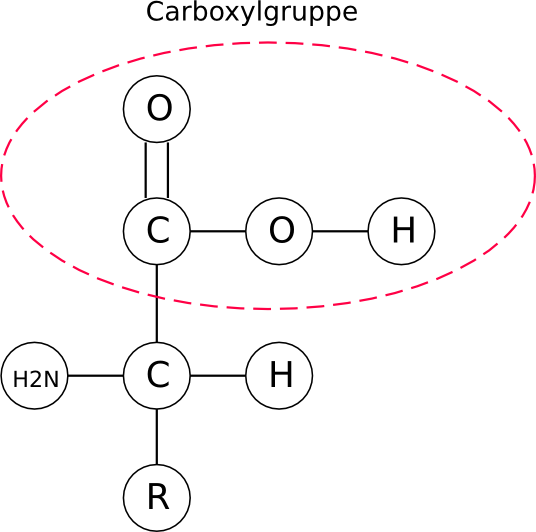
\includegraphics[scale=1]{image/3.png}
\newline
\newline
R ... Rest (z.B. Aminubutonsäure)
\newline
\newline
\subsubsection{Aufgaben der Proteine}

\begin{itemize}
\item Enzymatische Katalysator (Enzyme $\rightarrow$ Biokatalysator), viele Vorgänge im menschlichen Körper werden über Proteine / Eiweiß geregelt; Vitamine sind Enzyme, die nicht vom Körper selber produziert werden können

\item Transport: Hemoglobin $\rightarrow$ Transportstoffe für Sauerstoff (Eisen)

\item Bewegung: Proteine sind Hauptbestandteil des Muskelgewebes

\item Mechanische Stückfunktion: Kolagene; geben der Haut und Sehnen ihre Reißfestigkeit

\item Immunsystem: Antikörper sind hochspezialisierte  Proteine, die Fremdsubstanzen wie Viren, Bakterien oder Fremdzellen erkennen und binden können (Weißen Blutkörper); Bakterien vergiften; Viren zerstören Zellen; Fremdkörper können Krankheiten übertragen

\end{itemize}

\subsection{Fette}

Fette und fette Öle sind Ester des dreiwertigen Alkohols Glycerin mit drei, meist verschiedenen, Monocarbonsäuren, den Fettsäuren (Ester bedeutet eine Verbindung zwischen organischen Säuren und Alkhol (z.B. Propantriol bzw. Glyzerin und Methansäure).
\newline
\newline
Propantriol + Methansäure (Ameisensäure) = Fett

\newpage

\section{Gesundheit}

Richtige Ernährung
\newline
\newline
Ernährung heißt Energie zuführen. 
Energie kann auf verschiedene Form - in chemischer Form zugeführt werden
die Stoffe haben einen bestimmten Joule Wert 1k Kalorie = 4,2k Joule
\newline
\newline
Jetzt ist es so das man als ausgeachsenen mensc einen bestimmten joule verbraucht. weil es den betriebswert gi bt endoterm es muss energie zugeührt werden zusätlich kommt ein teil dazu wenn man aktiv ist (bewegung) 
\newline
\newline
Der Grundbedarf ist der Bedarf an Energie, die ein Mensch beim Sitzen oder Liegen verbraucht. Der Grundumsatz (=Grundbedarf) bei einem 70 Kilo Menschen ist in etwa 7000k Joule. Tätigkeitsumsatz kann bis zu 20000k Joule zusätzlich brauchen.
\newline
\newline
Der Mensch ist ein Heterotropher, der Mensch ist ein Allesfresser. Der Fettanteil sollte 25\% der Eingenommen Essen (hängt vom Verbrauch aus). Vitamine sind Stoffe, die der Körper nicht alleine herstellen kann.
\newline
\newline
Wichtige Vitamine:

\begin{itemize}
\item Vitamin A (Retinol)
\item Vitamin B1 (Thiamin)
\item Vitamin B2-Gruppe 
\item Vitamin B6 (Pyridxoin)
\item Vitamin B12 (Cobalamin)
\item Vitamin C
\item Vitamin D
\item Vitamin E (Fruchtbarkeisvitamin)
\item Vitamin K
\end{itemize}

\section{Gicht}

Harnssäurespiegel im Blut is zu groß und diese Harnsäure lagert sich in den gelenken an den schleimbeuteln und sehnen ab, Ursache ist das Burin, die kommt in tierischen Nahrungsmittel (Innerein, Hüllsenfrüchte). Sehr schmerzhaft. Hizegefühl. 

\section{Krankheitserregern}

Es gibt drei verschiedene Arten von Krankheitserreger.

\begin{itemize}
\item \textbf{Virus}: ist ein Stück der DNA und ist gebunden an eine Wirdszelle. Sie benötigen, um leben und vervielverltigen zu können lebende Zellen (Zellgebunden, aktive lebende Zellen). Das sie den Wirdzellen dazu bringen den Virus zu vermehren (Wirdszelle geht dabei zugrunde), zerstörung der Zelle | Kettenreaktion; im Blut können Antikörper gebildet werden, die den Virus binden können; aber gegen manche Viren ist das Immunsytem zu schwach (z.B. weil es durch den Virus angegriffen wird z.B. Aids) | kein Lebewesen (nur DNS)

\item \textbf{Bakterien}:  sind eine Vorstufe einer Zelle, haben alles aber nicht einen Zellkern, die DNS schwimmt im Plasma herum (in der Zelle) (=Prokaryonten), haben einen eigenen Stoffwechsel, können sich vermehren durch einfache Teilung (haben alle Merkmale eines Lebewesens); manche sind sogar beweglich (man unterscheidet sie von ihren Formen oder Farbstoffen Gram Positiv und Negative; nehmen sie Farbstoff auf oder nicht) ; Stäbchen förmige, Kugelbakterien (Koken), Spiralförmigen (spiroucheten/spirillen) die sind beweglich durch Schraub Bewegunggen. Bakterien halten sich meisten im Blut auf oder in Schleimhäuten und zwischen den Körperzellen. Dringen nicht (meistens) in die Zellen ein. Bakterien können durch Vergiftung den Körper schädigen.

\item \textbf{Pilze}: sind Pflanzen, ohne die Fähigkeit Fotossynthse zu betreiben, damit brauchen organische Nahrung z.B. Haut, ...

\item\textbf{Einzeller}: bestehen aus einer vollständigen Zelle (Kern + DNS + Hülle); Unterscheidung durch Form: Sporentierchen (Form: einfach Kugelzelle, unbeweglich), Wechseltierchen (Form: beliebig; Form ist veränderlich und dadurch können sie sich fortbewegen) (=Amöben genannt), Geiseltierchen (Form: haben einen Schwanz, beweglich), Wimperntierchen (=Pantoffeltierchen) (Form: länglich gezogen, hat Wimpern, beweglich).

\item \textbf{Parasiten}: mehrzellige Lebewesen (z.B. Bandwurm, Egel, Spulwürmer, ...)
\end{itemize}

\subsection{Krankheiten durch Viren}

\begin{itemize}
\item Aids: Erreger befällt das Immunsystem
\item Masern: merk man daran das man im Mund Flecken hat, hellrote Flecken hinter Ohren, ist selber harmlos, schwächt aber das Immunsystem
\item Windpocken: entstehen Bläschen auf der Haut, jucken
\item Mumps: befällt die Ohrspeicheldrüse
\item Röteln: sind ähnlich wie die Masern, kommt zu Schwellung der Nümpfknoten; Gefährlich bei schwangerne Frauen
\end{itemize}

Alle diese Krankheiten werden heute vorbeugend geimpft (Schutzimpfungen).

\subsubsection{Aids}
Aids ist ein Spezialfall der Virusimpfsektion. Führt letztlich zur Zerstörung des Immunsystem, man stirbt an Krankheiten, die das Immunsystem abwehren sollte.
\newline
\newline
Nicht jeder der sich ansteckt muss davon krank werden, es hängt von der Menge ab. Kaposi Sarkom = Hautkrebs meist verbunden mit Lungenerdzündung Polio (=Kinderlähmung) ist mittlerweile ausgestorben. Tollwut wird von Tieren übertragen, kann zum Tode führen.

\section{Bakterielle Krankheiten}

Diese Krankheiten sind behandelbar, umso länger die Erreger im Körper sind desto größer ist der Schaden. Die Pest ist ein Bakterieller Erreger (ist noch nicht Ausgerottet).

\subsection{der Tripper}
Der Tripper ist bei Männer spürbar und verursacht Entzündungen im Harnrohr. Bei der Frau oftmals nicht merkbar.

\subsection{Syphilis}
Syphilis wurde aus der neuen Welt eingeschleppt. 

\subsubsection{Der Verlauf der Erkrankung}

\begin{itemize}
\item nach 3 Wochen glattes Geschwür an der Infektionsstelle, schmerzlos, verschwindet wieder, Krankheitserreger, breiten sich über das Blut in den Körper 
\item nach 2 Monaten Hautausschlag der nicht schmerzt und nicht juckt, verschwindet auch von selber
\item innerhalb der nächsten 2 Jahre Ausschläge wiederholen sich, Haarausfall, Mundschleimhäute entzünden sich
\item nach 5 Jahren ist das Endstadium erreicht, lebenswichtige Organe werden angegriffen (Gehirn,...)
\end{itemize}

\subsection{Typhus}

Typhus: unkontrollierbarer Brechreiz und Durchfall (=Sarmonellen Vergiftung) ist Behandelbar.

\subsection{Thuberkulose Tbc}
Thuberkulose Tbc (Schwinsucht): Stäbchen Bakterien. Fürher sind 1/7 aller Menschen daran gestorben. Alle möglichen Organe werde befallen. Der Erreger wurde von Robert Koch (deutscher, 1843 - 1910) infiziert und benannt. Tröpcheninfektion (Lunge), leichte Grippe, wenn sie sich ausbreiten bilden sich im Körper Knoten (Körpertobulose), wenn man es übersteht ist man dagegen Immun. SpätTbc ist die nächste Stufe, offener Tbc, blutiger Auswurf, Husten. 
Krankheit des 19 Jahrhunderts.


\section{Einzeller als Krankheitserreger}

\subsection{Malaria}
Malaria (=Sumpffieber) - Erreger ist das Sporentierchen (=Plassmodium)
Auf der Erde gibt es ca. 3 Millionen Menschen, die darunter leiden. Übertragung durch Sumpfmücke (=Anopheles), die hat den Erreger im Speichel. Man hat versucht den Erträger zu bekämpfen, viele Städte trocken gelegt. Mit Flugzeugen haben sie über Sümpfe DDT (tötet die Mücke; Insektizide) gesprüht. DDT ist sehr langsam abbaubar, wurde in sehr vielen Lebensmittel weltweit nachgewiesen. Er befällt die Roten Blutkörperchen.

\subsubsection{Drei verschiedenen Verläufe}

\begin{itemize}
\item Terziär: 1 bis 2 Studen jeden dritten Tag hohes Fieber (40 Grad)
\item Quartiär: 3 bis 4 Stunden jeden vierten Tag hohes Fieber (40 Grad)
\item Tropika: unregelmäßig Fieber (40 Grad)
\end{itemize}

Gegenmittel: Chinin

\subsection{Schlafkrankheit}
Schlafkrankheit: Erreger: Trypanosma (=Geiseltierchen); wird von der CC-Flüge; sie überträgt den Erreger durch einen Stich; Erreger gelangt ins Blut und lagert sich an den Schleimhäuten an; lang anhaltende Schlafzustände; Tod dringt durch gifte Stoffe, die der tote Erreger absondert.
\newline
Parasiten z.B. Rinderbandwurm; es braucht einen Wirt und einen Zwischenwirt; der Organismus der die Geschlechtsreife trägt ist der Wirt; der der die Larvenform ist der Zwischenwirt; besteht aus einem Kopf mit Saugnäpfen und dann aus Gliedern, die nur Geschlechtsorgane dort entwickeln sich die Eier, hat davon viele viele; braucht keinen Geschlechtspanter; an diesen Gliedern entstehen die Eier; Infektionsweg der Mensch 

\newpage

\section{Ökologie}

Ist eine Wissenschaft über die Naturhalshauslehre. Was kommt hinein was kommt hinaus? Setzt sich aus verschiedenen Faktoren zusammen:

\begin{itemize}
\item unbelebte Faktoren:

	\begin{itemize}
	\item Wetter (Regen, Kälte, ...)
	\item Geografische Lage (Jahreszeiten, ...)
	\item Mondphasen
	\end{itemize}
	
\item belebten Faktoren

	\begin{itemize}
	\item andere Lebenswesen (Nahrungsbeschaffung, ...)
	\item Fortpflanzung
	\end{itemize}
	
\end{itemize}

Natürlicher Kreislauf (=Kohlenstoffkreislauf):

\begin{itemize}
\item Produzenten: sind die Pflanzen $\rightarrow$ O2, organische Substanzen
\item Konsument: sind die Tier (z.B. Schnecke) $\rightarrow$ CO2, NH3, organische Substanz
\item Destruenten: sind die Mikroorganismen $\rightarrow$ CO2 und Mineralstoffe
\end{itemize}

Es können zu Störung kommen: Den Pflanzen geht es zu gut $\rightarrow$ Algenexplosion, zu viel Mineralstoffe $\rightarrow$ Überdüngt. Mineralanreicherung $\rightarrow$ Algen sind Einzeller und können sich schnell fortpflanzen durch einfache Teilung. In der Nacht gibt es einen Sauerstoffmangel $\rightarrow$ die Pflanzen sterben. Die Mikroorganismen können es nicht zersetzen, da sie keinen Sauerstoff haben. Das Gewässer kippt $\rightarrow$ die Fäulnisbakterien scheiden Gifte Stoffe aus. Vergiftung, Überdüngung, Sauerstoffemangel, Anerober

\section{Nahrungsketten}

Def.: eine Nahrungsketten ist eine aufeinander folgen von Organismen, in der ''organische'' Stoffe weitergereicht wird. Die KEtte hat ein Anfang und ein Ende. Jede Nahrungskette beginnt mit den Produzenten, wenn der Mensch in der Kette beteiligt ist, ist er meistens das Ende. Der Nachteil des Kettenende ist das wenn Gift im Spiel ist, dieser am meisten davon trägt.- Einfach Nahrungskette: Gras, Kuh, Milch, Mensch.
\newline
\newline
Südwassersee in Südafrika:
\begin{itemize}
\item Stoffkreislauf
\item 
\end{itemize}

Beispiel DDT in der Nahrungskette:
\newline
0,01 ppm DDT
0,33 ppm Algen
0,42 ppm Muscheln
2,00 ppm Hecht
2500 Eier (Vögel)
250000 fach
\newline

1 SR 90
730 Muscheln
950 
3000 Hecht
3500 Bisamratte
\newline
Nicht abbaubar, wird gespeichert statt dem Kalzium. Halbwertszeit kommt nicht zur Geltung, Konzentration steigt an.


Phosphor33 - Plfanzen nehmen das gierig auf
300000 Algen (Pflanzen sind wild nach Phosphor)
100000 Einzeller (werden ausgeschieden oder durch die Halbwertszeit zerfallen)
100000 Fische

\end{document}